\documentclass[english,onecolumn]{scrartcl}
\usepackage[T1]{fontenc}
\usepackage{listings}
\usepackage{hyperref}
\usepackage{tabularx}
\usepackage{multirow}
\usepackage{tikz-timing}
\usepackage{graphicx}
\usepackage{pdfpages}
\usepackage[style=ieee, backend=biber]{biblatex}

\definecolor{darkgreen}{HTML}{008000}
\lstset{frame=single,
    language=Haskell,
    breaklines=true,
    showspaces=false,
    showstringspaces=false,
    showtabs=false,
    commentstyle=\color{darkgreen},
    keywordstyle=\color{blue},
    stringstyle=\color{purple},
    title=\lstname}
\def\tabularxcolumn#1{m{#1}}
\pagenumbering{roman}
\tikzset{timing/draw grid}
\addbibresource{references.bib}

\begin{document}
\title{ECE4095 Final Report}
\subtitle{H2V --- a Haskell to Verilog Compiler}
\author{Reuben D'Netto (22096620)}

\maketitle
\tableofcontents{}
\pagebreak{}
\pagenumbering{arabic}


\section{Significant Contributions}
\begin{itemize}
    \item Designed and implemented a Haskell to Verilog compiler
    \item Designed and implemented support for the following functions through a combination of generated and hard-coded Verilog:
        \begin{itemize}
            \item List operators: cons (:), concat (++)
            \item Higher order list functions: map, fold/reduce, zipWith
        \end{itemize}
    \item Designed and implemented support for N-degree parallel computation of lists, as defined by user
    \item Designed and implemented support for evaluation of higher order functions at compile-time
    \item Designed and implemented data flow graph generation
    \item Verified hardware generated for test cases using SignalTap
\end{itemize}


% Include poster such that it appears in the TOC without adding a heading to the page
% Code taken from: http://tex.stackexchange.com/questions/68272/make-section-headings-invisible
\newcommand\invisiblesection[1]{%
    \refstepcounter{section}%
    \addcontentsline{toc}{section}{\protect\numberline{\thesection}#1}%
    \sectionmark{#1}}

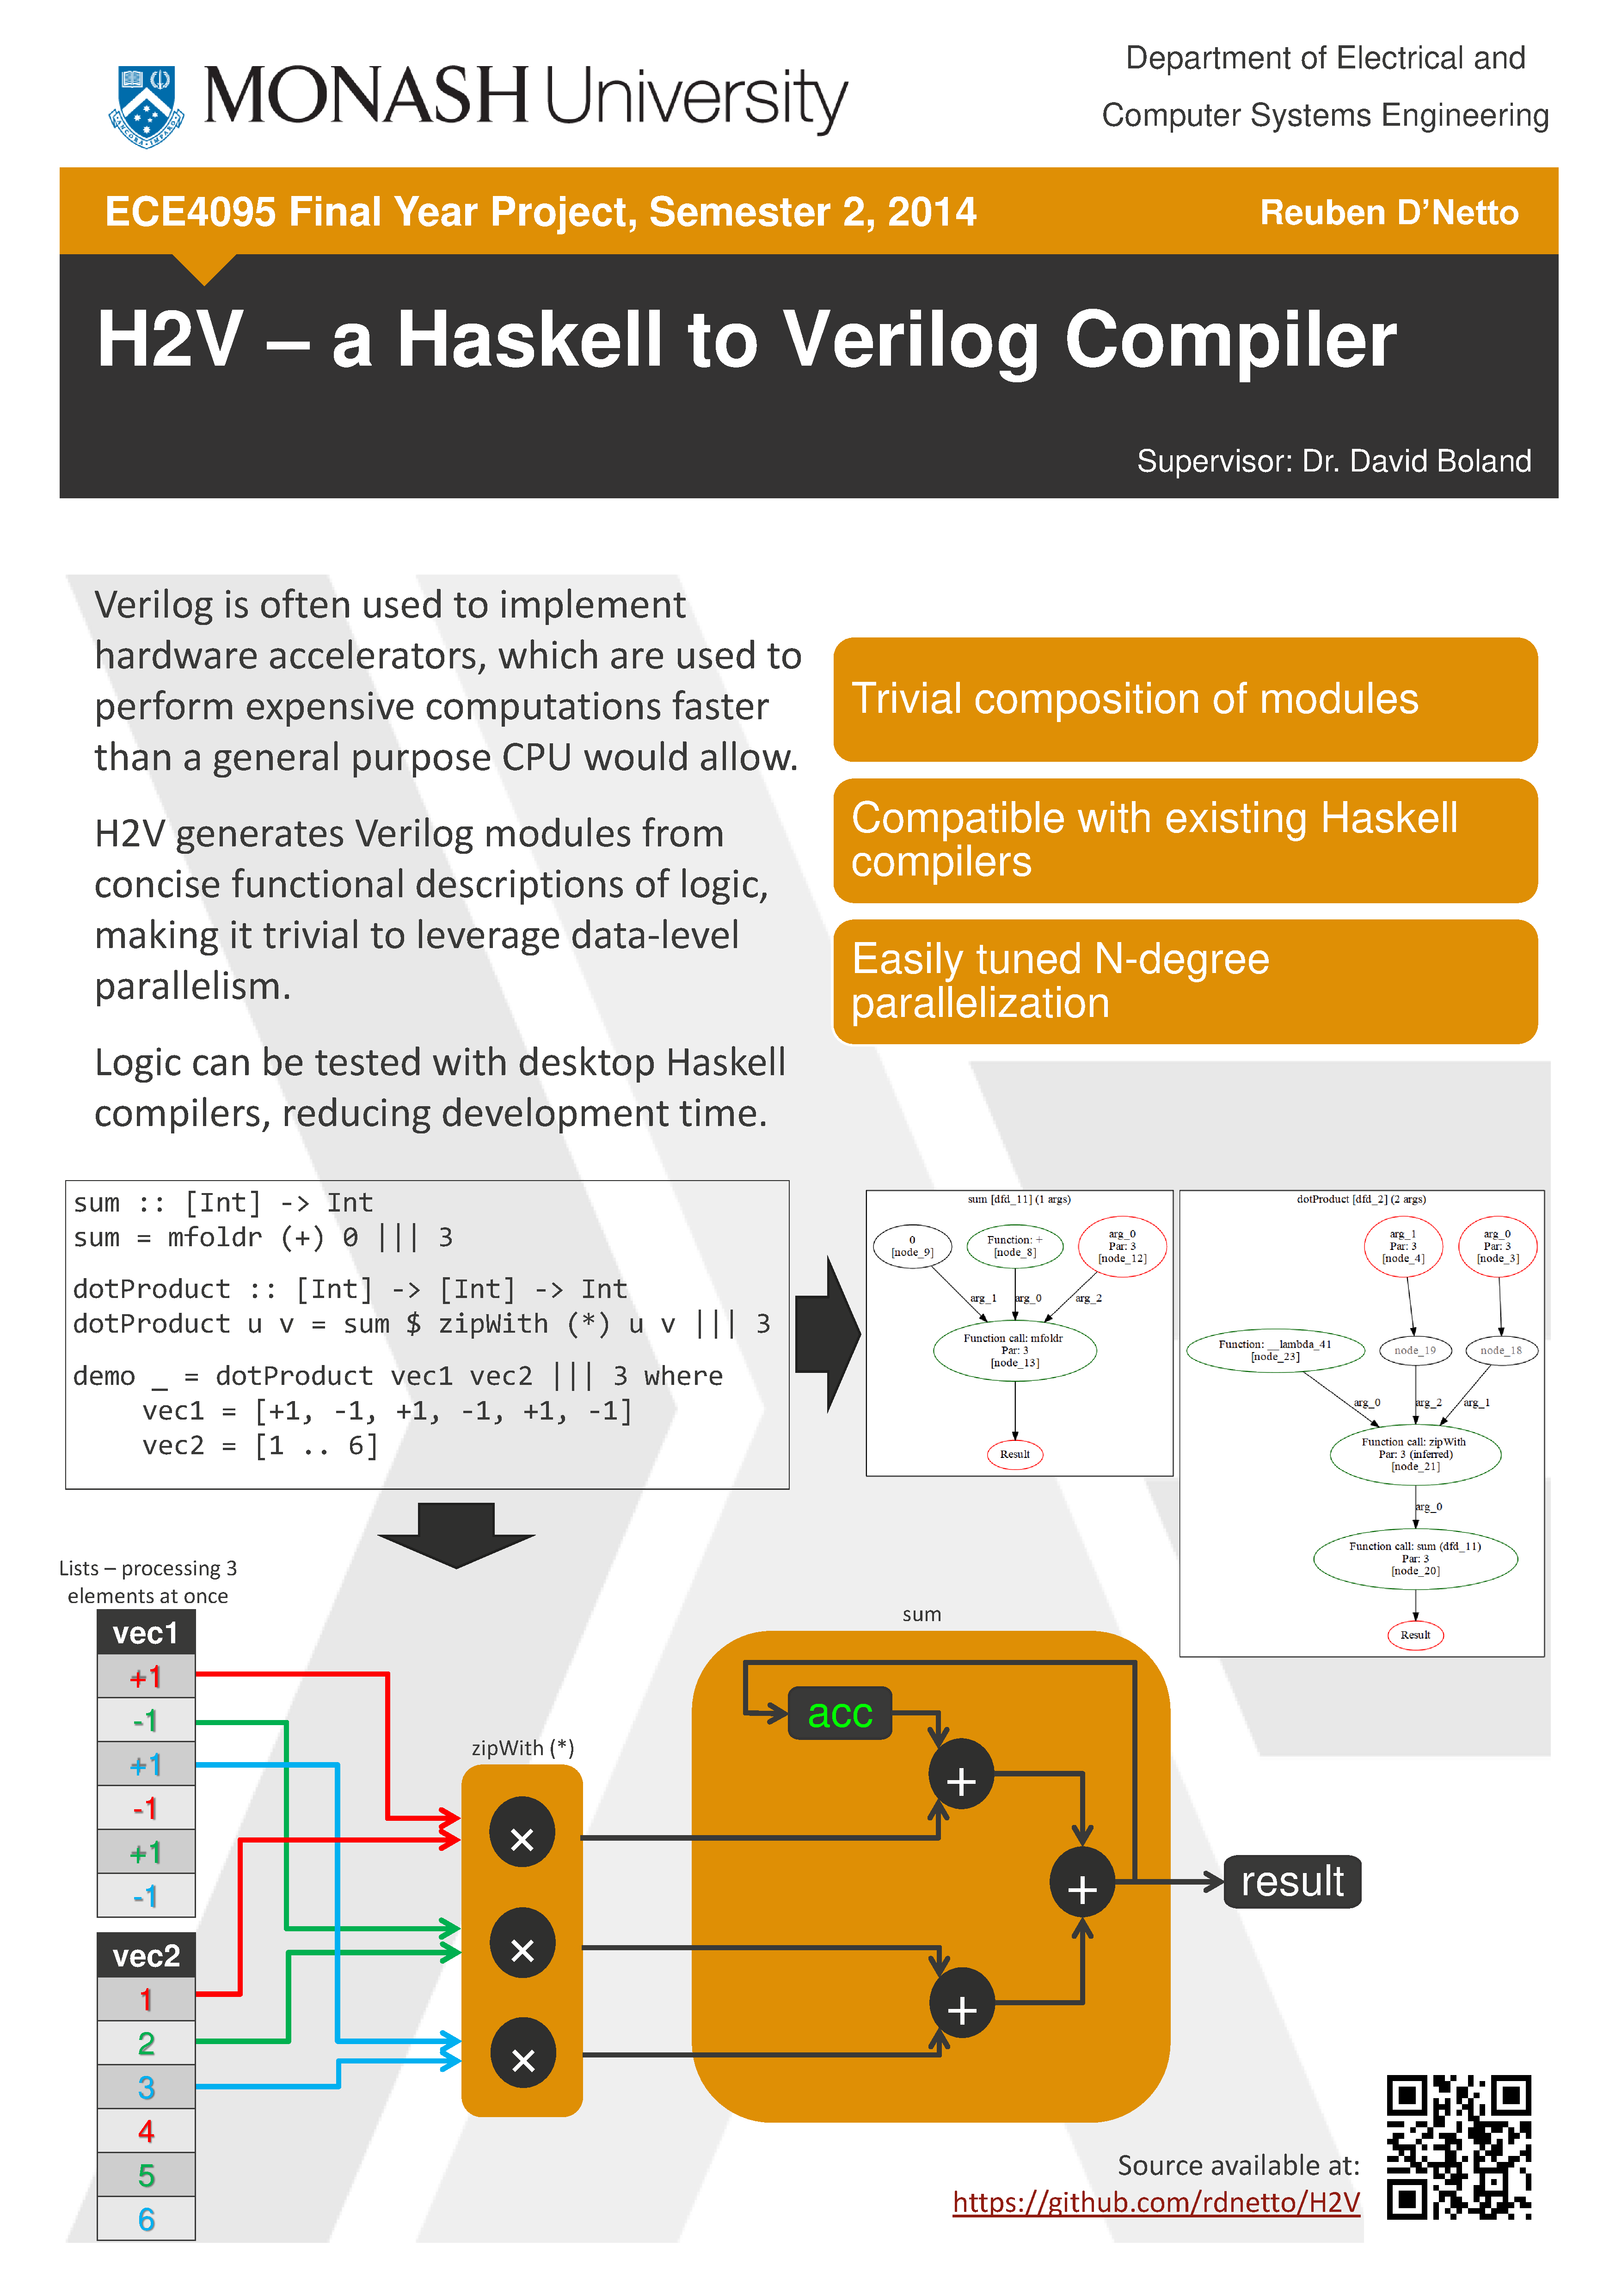
\includepdf[pages={1}, pagecommand={\invisiblesection{Poster}}]{../Poster/Poster.pdf}


\section{Introduction}
% TODO


\section{Supported Features}
% TODO


\section{Future Work}
% TODO



\appendix
\section{Appendix --- Test Cases}
\subsection{Language Features}
\lstinputlisting{../../H2V/tests/f0.hs}
\lstinputlisting{../../H2V/tests/f1.hs}
\lstinputlisting{../../H2V/tests/guards.hs}
\lstinputlisting{../../H2V/tests/pattern_match.hs}
\lstinputlisting{../../H2V/tests/fib.hs}

\subsection{Higher Order Functions}
\lstinputlisting{../../H2V/tests/ho_arg.hs}
\lstinputlisting{../../H2V/tests/ho_flip.hs}
\lstinputlisting{../../H2V/tests/ho_pa.hs}
\lstinputlisting{../../H2V/tests/ho_return.hs}

\subsection{Lists}
\lstinputlisting{../../H2V/tests/lists.hs}
\lstinputlisting{../../H2V/tests/lists2.hs}
\lstinputlisting{../../H2V/tests/demo.hs}

\section{Appendix --- Source Code}
\lstinputlisting{../../H2V/main.hs}
\lstinputlisting{../../H2V/Common.hs}
\lstinputlisting{../../H2V/DfdDef.hs}
\lstinputlisting{../../H2V/GenerateDFD.hs}
\lstinputlisting{../../H2V/RenderGraphviz.hs}
\lstinputlisting{../../H2V/RenderVerilog.hs}
\lstinputlisting{../../H2V/AST_Display.hs}

\section{Appendix --- Include Files for H2V Programs}
\lstinputlisting{../../H2V/include/hs/H2V_Compat.hs}
\lstinputlisting{../../H2V/include/v/include.v}

\printbibliography

\end{document}

